\documentclass[letterpaper]{article}

\usepackage{tbil-la}
  %\booltrue{TR}   %Drew
  \boolfalse{TR}  %Steven

% 
\usepackage{tbil-la}

\usepackage[top=1in,bottom=1in,left=1in,right=1in]{geometry}
\usepackage{enumerate,hyperref}
\pagestyle{empty}

\begin{document}




\begin{center}
{\Large \bf Office Hours Reassessment Form} \\
\large \course
\end{center}



\vspace{0.2in}

\begin{flushleft}
{\bf Name: } \underline{\phantom{xxxxxxxxxxxxxxxxxxxxxxxxxxxxxxxxxxxxxxxxxxxxxxxxxxxxxxxxx}} \\
\vspace{0.15in}
{\bf Date: } \underline{\phantom{xxxxxxxxxxxxxxxxxxxxxxxxxxxxxxxxxxxxxxxxxxxxxxxxxxxxxxxxx}} \\
\vspace{0.15in}
{\bf Standard: } \underline{\phantom{xxxxxxxxxxxxxxxxxxx}} \\
\vspace{0.15in}
{\bf Assessment marked with \reattemptMark{}: } \underline{\phantom{xxxxxxxxxxxxxxxxxxxxxxxxxxxxx}} \\
\vspace{0.15in}
{\bf List of practice problems worked: } \\
\vspace{0.4in}
Use this space to show your work on at least {\bf three} practice problems.  Use the back and/or attach additional pages as necessary.

\vfill

\vspace{0.15in}
{\bf Result of reassessment: } \underline{\phantom{xxxxxxxxxxxxxxxxxxxxxxx}} \\

\end{flushleft}

\end{document}



\usepackage{tbil-la}

\usepackage[top=1in,bottom=1in,left=1in,right=1in]{geometry}
\usepackage{enumerate,hyperref}
\pagestyle{empty}

\begin{document}




\begin{center}
{\Large \bf Reassessment Form (\reattemptMark{})} \\
\large \course{} - \prof
\end{center}



\vspace{0.2in}

\begin{flushleft}
{\bf Name: } \underline{\phantom{xxxxxxxxxxxxxxxxxxxxxxxxxxxxxxxxxxxxxxxxxxxxxxxxxxxxxxxxx}} \\
\vspace{0.15in}
{\bf Date: } \underline{\phantom{xxxxxxxxxxxxxxxxxxxxxxxxxxxxxxxxxxxxxxxxxxxxxxxxxxxxxxxxx}} \\
\vspace{0.15in}
{\bf Standard: } \underline{\phantom{xxxxxxxxxxxxxxxxxxx}} \\
\vspace{0.15in}
{\bf Assessment marked with \reattemptMark{}: } \underline{\phantom{xxxxxxxxxxxxxxxxxxxxxxxxxxxxx}} \\
\vspace{0.15in}
{\bf List of practice problems worked: } \\
\vspace{0.4in}
Use this space to show your work on at least {\bf three} practice problems.  Use the back and/or attach additional pages as necessary. Bring this form
to office hours to be given an opportunity to work a new problem.

\vfill

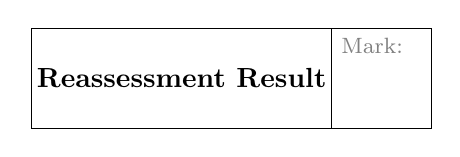
\begin{tikzpicture}[x=0.5in,y=0.5in]
  \draw (0,0) rectangle (4,1);
  \draw (3,0) -- (3,1);
  \node at (1.5,0.5) {\textbf{Reassessment Result}};
  \node[anchor=north west] at (3,1) {\footnotesize\textcolor{gray}{Mark:}};
\end{tikzpicture}

\end{flushleft}

\newpage

\begin{center}
{\Large \bf Reassessment Form (\minorMark{})} \\
\large \course{} - \prof
\end{center}



\vspace{0.2in}

\begin{flushleft}
{\bf Name: } \underline{\phantom{xxxxxxxxxxxxxxxxxxxxxxxxxxxxxxxxxxxxxxxxxxxxxxxxxxxxxxxxx}} \\
\vspace{0.15in}
{\bf Date: } \underline{\phantom{xxxxxxxxxxxxxxxxxxxxxxxxxxxxxxxxxxxxxxxxxxxxxxxxxxxxxxxxx}} \\
\vspace{0.15in}
{\bf Standard: } \underline{\phantom{xxxxxxxxxxxxxxxxxxx}} \\
\vspace{0.15in}
{\bf Assessment marked with \minorMark{} (include version): } \underline{\phantom{xxxxxxxxxxxxxxxxxxxxxxxxxxxxx}} \\
\vspace{0.15in}
Use this space to completely rework the problem. (This form is due the next
class day following when the marked assessment was returned.)

\vfill

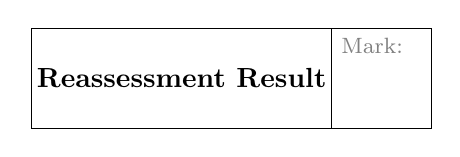
\begin{tikzpicture}[x=0.5in,y=0.5in]
  \draw (0,0) rectangle (4,1);
  \draw (3,0) -- (3,1);
  \node at (1.5,0.5) {\textbf{Reassessment Result}};
  \node[anchor=north west] at (3,1) {\footnotesize\textcolor{gray}{Mark:}};
\end{tikzpicture}

\end{flushleft}

\newpage

\end{document}
